%%Template made by Uday Khankhoje for examinations using the exam template
%%Refer to the documentation http://www-math.mit.edu/~psh/exam/examdoc.pdf 
%%for lot more bells and whistles to the standard template shown below
\documentclass[a4paper,11pt,addpoints]{exam}
\usepackage[left=1.5cm,right=1.5cm,top=1.5cm,bottom=2cm]{geometry}
%\usepackage{mathrsfs}
\usepackage{graphicx,color}
\usepackage[x11names]{xcolor}
\usepackage{venndiagram}
\usepackage{epic,eepic}
%\usepackage{mathpazo}
\usepackage{url}
\usepackage{tasks} % cria lista curta
\usepackage{multicol}
\usepackage{amsmath, amsthm, amssymb}
\pointsinmargin
\boxedpoints 
\renewcommand*\half{.5}
\usepackage{setspace}
\DeclareMathOperator{\vecc}{vec}
%\renewcommand{\vec}[1]{\ensuremath{\mathbf{#1}}}

\global\vbadness=1616

\begin{document}
\noindent 
%%PART 1 of header
\begin{center}
	\vspace*{-3em}
\def\arraystretch{2.0}
\begin{tabular}{|p{0.7\linewidth}|p{0.2\linewidth}|}
\hline 
\textbf{Atividade de Matemática - Primeiro Bimestre} & Pontos Obtidos $\downarrow$ \\
\hline 
Data:\hspace{3cm}  Total de questões \textbf{\numquestions} \hspace{1cm} Total de pontos: \textbf{\numpoints} &   \\ 
\hline 
\multicolumn{2}{|l|}{Tuma: \hspace{0.3\linewidth} Nome: \hspace{0.3\linewidth} Duração: 2 hrs} \\
\hline
\end{tabular} 
\end{center}
%%PART 2 of header, if you have too many questions, this may be a problem
%%if so, use \multirowgradetable{n}[questions], where n is the number of rows you want
%%or, switch to \gradetable[h][pages] instead, 
\begin{center}
\gradetable[h][questions]
\end{center}
%%PART 3 of header
\textbf{Instruções
\begin{enumerate}
    \item Explique todas as questões claramente.
    \item Necessário todos os cálculos.
\end{enumerate}
}
%%toggle comment on next line to show/hide the answers
% \printanswers
%%Now the actual paper!
\begin{questions}
\question[2] 
Um terreno tem a forma de um triângulo retângulo. Algumas de suas medidas estão indicadas, em metros, na figura. 
Determine as medidas de \textbf{x} e \textbf{y} dos lados desse terreno.

\begin{figure}[htb!]
  \centering
  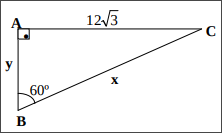
\includegraphics[width=.3\linewidth]{figures/img1.png}
\end{figure}

\question[2] 
Calcule a soma dos catetos do triângulo retângulo da figura, sabendo que $AB = 10$ e $BC = 6$.


\begin{figure}[htb!]
  \centering
  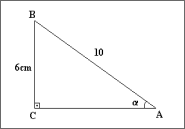
\includegraphics[width=.3\linewidth]{figures/img2.png}
\end{figure}

\begin{tasks}(5)
  \task 6
  \task 8
  \task 14
  \task 2
  \task 16
\end{tasks}

\question[2]

Transforme em radianos as seguintes medidas de arcos em graus.

\begin{tasks}(2)
  \task $30^{\circ}$
  \task $300^{\circ}$
  \task $1080^{\circ}$
  \task $235^{\circ}$
  \task $20^{\circ}$
  \task $150^{\circ}$
\end{tasks}

\question[4]

Calcule o valor de:

\begin{tasks}(2)
  \task $\cos 210^\circ$
  \task $\sin 120^\circ$
  \task $\tan 330^\circ$
  \task $\tan 210^\circ$
  \task $\cos 300^\circ$
  \task $\sin 300^\circ$
  \task $\cos 1200^\circ$
  \task $\cos 1575^\circ$
  \task $\sin 4200^\circ$
  \task $\sin \frac{2\pi}{3}$
\end{tasks}


\end{questions}
\end{document}
